\section{Propagation sur les lignes de transmission}
Dans le cas des signaux basses fréquences (BF) utilisés dans les circuits
électroniques, la longueur d'onde $\lambda = c/f$ est extrêmement grande
($\lambda = 30$~km à 1~kHz). A circuit BF can therefore be treated as a set of
éléments localisés joined by ideal wires: dans l'approche de l'électronique BF,
la tension aux bornes de la charge est considérée égale à la tension de la
source de manière instantanée. At radio frequency this fails. Pour les signaux
radiofréquences (RF), la longueur d'onde est petite ($\lambda = 30$~cm à 1~GHz
et 3~mm à 100~GHz) et par conséquent, la taille des composants électroniques,
la longueur des pistes sur les circuits imprimés et la longueur des câbles
deviennent alors non négligeables par rapport à $\lambda$. L'importance de la
valeur relative de $\lambda$ (par rapport aux dimensions globales des circuits)
explique ainsi la raison pour laquelle les circuits RF ne peuvent pas être
traités de la même manière que les circuits BF en termes d'analyse, de
conception, de fabrication et de caractérisation. La théorie des lignes de
transmission s'applique alors aux pistes, aux câbles et plus généralement aux
circuits et systèmes RF.

\subsection{Définition d'une ligne de transmission}
\begin{definition}[Ligne de transmission (\textit{transmission line})]
  Le terme de \textbf{ligne de transmission} s'applique à certains éléments
  utilisés en ingénierie RF dont les dimensions sont du même ordre de grandeur
  que la longueur d'onde $\lambda$. Il existe différents types de lignes de
  transmission, qui se distinguent par le nombre de conducteurs métalliques
  qu'elles comportent (1, 2 ou 3 conducteurs métalliques).
\end{definition}

\subsubsection{Lignes de transmission à 1 conducteur métallique}
Les lignes comportant 1 unique conducteur métallique sont les \textbf{guides
d'ondes} (\textit{waveguide}) métalliques, qui peuvent être de forme
rectangulaire ou circulaire. Parmi les différents types de lignes de
transmission utilisées en ingénierie RF, les guides d'ondes présentent le plus
\emph{faible} affaiblissement et supportent la plus \emph{forte} puissance : ils
sont donc les mieux adaptés aux applications où l'affaiblissement des signaux
devient très élevé (typiquement, aux fréquences supérieures à 30~GHz), dans les
radars civils ou militaires, les communications satellites et les systèmes RF.
Les guides d'ondes sont de fait employés dans des situations qui ne seront pas
étudiées dans ce cours.

\subsubsection{Lignes de transmission à 2 conducteurs métalliques}
Les lignes comportant 2 conducteurs métalliques sont principalement les
\textbf{câbles coaxiaux} (\textit{coaxial cable}) et les lignes sur circuits
imprimés appelées \textbf{lignes microruban} (\textit{microstrip line}) ou
lignes microstrip. Les 2 conducteurs métalliques sont séparés par un matériau
diélectrique caractérisé par sa permittivité relative $\varepsilon_r$ (ou
constante diélectrique). La perméabilité relative est $\mu_r = 1$.

Pour un câble coaxial, le conducteur interne transporte le signal RF tandis que
le conducteur externe est la référence connectée à la masse (notée GND). Pour
une ligne microruban, c'est le conducteur supérieur qui transporte le signal RF
tandis que le conducteur inférieur constitue le \textbf{plan de masse}
(\textit{ground plane}). Les câbles coaxiaux et les lignes microruban sont les
lignes de transmission les plus fréquemment utilisées en ingénierie RF et par
conséquent, il est fondamental d'étudier leurs propriétés et caractéristiques.

\begin{example}[Diélectriques typiques]
  Un câble coaxial ayant pour matériau diélectrique du Téflon a
  $\varepsilon_r = 2{,}1$ ; le Téflon est en fait une marque déposée qui
  correspond au PolyTétraFluoroÉthylène (PTFE). Un filtre passe-bas (LPF)
  entièrement réalisé avec des lignes microruban gravées sur de l'Alumine a
  $\varepsilon_r = 9{,}8$. Dans ces 2 exemples, les conducteurs métalliques sont
  constitués de cuivre.
\end{example}

\paragraph{Câble coaxial}
Dans un câble coaxial, les champs $\v{E}$ et $\v{H}$ sont orthogonaux entre eux
et sont également orthogonaux à la direction de propagation : on retrouve alors
le mode de propagation TEM (transverse électrique et magnétique). Puisque les
champs se propagent uniquement \emph{à l'intérieur} du câble coaxial, le
rayonnement de puissance est fortement limité vers l'extérieur. Par défaut, on
dira qu'il est donc isolé d'un point de vue électromagnétique : c'est le
\textbf{blindage électromagnétique} (\textit{electromagnetic shielding}). Un
câble coaxial peut donc être facilement utilisé à proximité d'autres câbles
coaxiaux, d'un appareil de mesure, d'une surface métallique, être posé au sol,
tenu dans une main, sans interférences de la propagation du signal RF dans le
câble.

\paragraph{Ligne microstrip}
Pour les lignes microruban, les champs se propagent à la fois dans le matériau
diélectrique et dans l'air : le milieu de propagation est donc
\textbf{inhomogène} (\textit{inhomogeneous}). Les champs $\v{E}$ et $\v{H}$
possèdent une faible composante longitudinale (c'est-à-dire, le long de la
direction de propagation) : c'est le mode de propagation \textbf{quasi-TEM}.
Cependant, les composantes longitudinales des champs sont si faibles que l'on
peut considérer que le mode de propagation est TEM.

Puisque les champs se propagent en partie dans l'air, les lignes microruban ont
donc tendance à rayonner de la puissance vers l'extérieur, contrairement aux
câbles coaxiaux. Cette propriété peut être vue comme un avantage ou un
inconvénient. Le rayonnement des lignes microruban permet de les utiliser pour
concevoir des \emph{antennes} microruban ; mais pour les \emph{circuits} RF,
cela devient un inconvénient car la puissance rayonnée est alors diffusée dans
l'air, ce qui entraîne un affaiblissement plus important par rapport à un câble
coaxial de même longueur ainsi que la perturbation potentielle du fonctionnement
d'autres circuits situés à proximité.

\begin{figure}[h!]
  \centering
  \begin{tikzpicture}[scale=1.0]
    % coaxial cross-section
    \begin{scope}
      \fill[gray!10] (0,0) circle (1.3);
      \draw[very thick] (0,0) circle (1.3);
      \draw[very thick,fill=gray!50] (0,0) circle (0.3);
      \foreach \ang in {30,120,210,300}
        {\draw[->,thick] (\ang:0.32) -- (\ang:1.26);}
      \draw[dashed,gray] (0,0) circle (0.85);
      \draw[->,thick,gray] (75:0.85) arc (75:35:0.85);
      \draw[->,thick,gray] (255:0.85) arc (255:215:0.85);
      \draw[|<->|] (0,-1.6) -- node[below,font=\scriptsize,inner sep=1pt] {$b$} (-1.3,-1.6);
      \draw[|<->|] (0,-1.6) -- (0.3,-1.6);
      \node[font=\scriptsize,anchor=west,inner sep=2pt] at (0.34,-1.6) {$a$};
      \draw[gray,thin] (0,-1.3) -- (0,-1.68);
      \node[font=\scriptsize,anchor=west] at (1.45,0.75) {$\v{E}$ radial};
      \node[font=\scriptsize,anchor=west] at (1.45,0.25) {$\v{H}$ azimutal};
      \node[font=\scriptsize] at (0.62,-0.32) {$\varepsilon,\mu$};
      \node[font=\scriptsize,align=center] at (0,-2.4)
        {câble coaxial : TEM,\\ blindage électromagnétique};
    \end{scope}
    % microstrip cross-section
    \begin{scope}[xshift=6.6cm,yshift=-0.35cm]
      \fill[gray!10] (-1.7,0) rectangle (1.7,0.8);
      \draw (-1.7,0) rectangle (1.7,0.8);
      \draw[very thick,fill=gray!50] (-0.4,0.8) rectangle (0.4,0.96);
      \draw[very thick] (-1.7,0) -- (1.7,0);
      \draw[thick] (0.4,0.88) .. controls (1.0,0.88) and (1.1,0.5) .. (1.1,0);
      \draw[thick] (0.4,0.96) .. controls (1.35,1.25) and (1.6,0.6) .. (1.6,0);
      \draw[thick] (-0.4,0.88) .. controls (-1.0,0.88) and (-1.1,0.5) .. (-1.1,0);
      \draw[thick] (-0.4,0.96) .. controls (-1.35,1.25) and (-1.6,0.6) .. (-1.6,0);
      \node[font=\scriptsize] at (0,0.4) {$\varepsilon_r,\ \mu_r=1$};
      \node[font=\scriptsize,anchor=south] at (0,1.3) {air};
      \node[font=\scriptsize,anchor=south] at (0,1.0) {conducteur (signal RF)};
      \node[font=\scriptsize,anchor=north] at (0,-0.08) {plan de masse (GND)};
      \node[font=\scriptsize,align=center] at (0,-2.05)
        {ligne microruban : quasi-TEM,\\ milieu inhomogène, rayonnement};
    \end{scope}
  \end{tikzpicture}
  \caption*{\small Cross-sections of the two lignes à 2 conducteurs. In the
  câble coaxial the radial $\v{E}$ and the azimuthal $\v{H}$ are entirely
  confined between the conducteurs; in the ligne microruban part of the field
  closes through the air.}
\end{figure}

\subsection{Modèle électrique d'une ligne de transmission}
Une ligne microruban ou un câble coaxial peuvent être modélisés à l'aide d'un
circuit électrique équivalent composé d'éléments résistif $R$, inductif $L$,
conductif $G$ et capacitif $C$. Ce circuit équivalent, dit \textbf{modèle
électrique ou RLGC}, possède une longueur considérée comme quasi nulle,
$dz \to 0$, et par conséquent, une ligne de transmission de longueur $L$ est
modélisée par une infinité de circuits RLGC en cascade.

\begin{notation}
  Étant donné que $dz \to 0$, les éléments $R$, $L$, $G$, $C$ sont des
  \textbf{éléments distribués} (\textit{distributed elements}), par opposition
  à des \textbf{éléments localisés} (\textit{lumped elements}) : ils sont
  définis \emph{par unité de longueur}.
  \begin{center}
    \begin{tabular}{llll}
      \toprule
      $R$ & résistance par unité de longueur  & $\Omega/\mathrm{m}$ & pertes métalliques\\
      $L$ & inductance par unité de longueur  & $\mathrm{H}/\mathrm{m}$ & magnetic energy\\
      $G$ & conductance par unité de longueur & $\mathrm{S}/\mathrm{m}$ & pertes diélectriques\\
      $C$ & capacité par unité de longueur & $\mathrm{F}/\mathrm{m}$ & electric energy\\
      \bottomrule
    \end{tabular}
  \end{center}
\end{notation}

La résistance par unité de longueur $R$ est due à la conductivité $\sigma$ non
infinie (ou la résistivité $\rho = 1/\sigma$ non nulle) des conducteurs
métalliques de la ligne de transmission. L'inductance par unité de longueur $L$
modélise le fait qu'un courant qui circule dans un conducteur métallique crée
un champ magnétique. La capacité par unité de longueur $C$ s'explique par le
fait qu'il y a 2 conducteurs métalliques à un potentiel différent et séparés
par un matériau diélectrique : il existe donc un champ électrique entre les 2
conducteurs métalliques. Les matériaux diélectriques isolants ne sont pas
parfaitement isolants et ils présentent des pertes. Ces pertes dans les
matériaux diélectriques sont modélisées par la conductance par unité de
longueur $G$.

\begin{prop}[Ligne sans pertes (\textit{lossless line})]
  Les éléments $R$ et $G$ du modèle équivalent sont responsables des pertes
  (atténuation notée $\alpha$) dans les lignes microruban et les câbles
  coaxiaux : $R$ est à l'origine des pertes dans les conducteurs métalliques,
  tandis que $G$ est à l'origine des pertes dans le matériau diélectrique.
  Ainsi, il est souhaitable pour une ligne de transmission de présenter une
  faible résistance par unité de longueur $R$ et une faible conductance par
  unité de longueur $G$, et
  \[\text{\textbf{lossless (ideal) line}} \iff R = 0 \text{ and } G = 0.\]
\end{prop}

\begin{remark}[Why copper, and why Teflon or air]
  Le cuivre ($\sigma = 58{,}7\times 10^{6}$~S/m) et l'aluminium
  ($\sigma = 36{,}9 \times 10^{6}$~S/m), qui font partie des métaux ayant la
  conductivité la plus élevée, sont presque exclusivement utilisés comme
  conducteur métallique dans les lignes microruban et les câbles coaxiaux. L'or
  est également un très bon conducteur ($\sigma = 41 \times 10^{6}$~S/m) mais
  le prix est bien trop élevé pour être massivement utilisé dans les câbles et
  circuits RF. Quant au choix du matériau diélectrique, il est fonction de
  nombreux paramètres et n'est pas uniquement guidé par la recherche de pertes
  diélectriques minimales. Si en pratique ce choix est assez vaste pour les
  lignes microruban, il est beaucoup plus limité pour les câbles coaxiaux où le
  Téflon ($\tan\delta = 5\times 10^{-4}$) et l'air ($\tan\delta = 0$) sont
  principalement utilisés. L'air sec est ainsi le matériau diélectrique qui
  présente les plus faibles pertes et il est systématiquement présent dans les
  câbles coaxiaux fonctionnant à des fréquences supérieures à environ 25~GHz.
\end{remark}

\begin{figure}[h!]
  \centering
  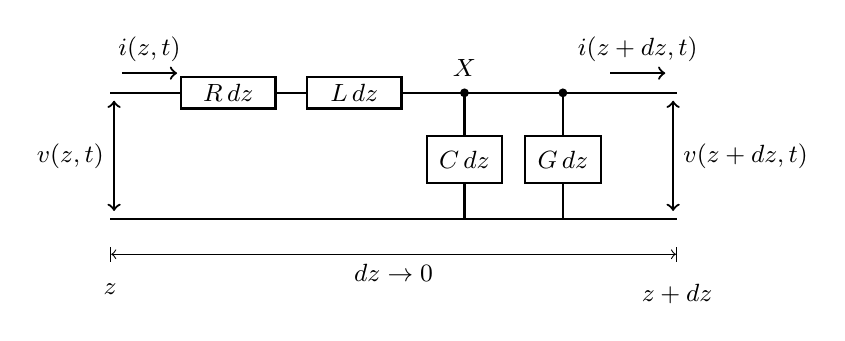
\begin{tikzpicture}[scale=1.0]
    % top wire with R dz and L dz
    \draw[thick] (-1.2,1.6) -- (-0.3,1.6);
    \draw[thick,fill=white] (-0.3,1.4) rectangle (0.9,1.8);
    \node[font=\small] at (0.3,1.6) {$R\,dz$};
    \draw[thick] (0.9,1.6) -- (1.3,1.6);
    \draw[thick,fill=white] (1.3,1.4) rectangle (2.5,1.8);
    \node[font=\small] at (1.9,1.6) {$L\,dz$};
    \draw[thick] (2.5,1.6) -- (6.0,1.6);
    % shunt branches
    \draw[thick] (3.3,1.6) -- (3.3,1.05);
    \draw[thick,fill=white] (2.82,0.45) rectangle (3.78,1.05);
    \node[font=\small] at (3.3,0.75) {$C\,dz$};
    \draw[thick] (3.3,0.45) -- (3.3,0.0);
    \draw[thick] (4.55,1.6) -- (4.55,1.05);
    \draw[thick,fill=white] (4.07,0.45) rectangle (5.03,1.05);
    \node[font=\small] at (4.55,0.75) {$G\,dz$};
    \draw[thick] (4.55,0.45) -- (4.55,0.0);
    \fill (3.3,1.6) circle (1.6pt);
    \fill (4.55,1.6) circle (1.6pt);
    \node[font=\small,anchor=south] at (3.3,1.68) {$X$};
    % bottom wire
    \draw[thick] (-1.2,0.0) -- (6.0,0.0);
    % ports
    \draw[->,thick] (-1.05,1.85) -- (-0.35,1.85);
    \node[font=\small,anchor=south] at (-0.7,1.87) {$i(z,t)$};
    \draw[->,thick] (5.15,1.85) -- (5.85,1.85);
    \node[font=\small,anchor=south] at (5.5,1.87) {$i(z+dz,t)$};
    \draw[<->,thick] (-1.15,1.5) -- node[left,font=\small] {$v(z,t)$} (-1.15,0.1);
    \draw[<->,thick] (5.95,1.5) -- node[right,font=\small] {$v(z+dz,t)$} (5.95,0.1);
    % axis
    \draw[|<->|] (-1.2,-0.45) -- node[below,font=\small] {$dz \to 0$} (6.0,-0.45);
    \node[font=\small,anchor=north] at (-1.2,-0.7) {$z$};
    \node[font=\small,anchor=north] at (6.0,-0.7) {$z+dz$};
  \end{tikzpicture}
  \caption*{\small The elementary RLGC cell. The loi des mailles is applied to
  the loop, the loi des nœuds to the nœud between the series and the shunt
  branch.}
\end{figure}

\subsubsection{Les éléments L et C pour un câble coaxial sans perte}
Pour un câble coaxial, les champs restent confinés à l'intérieur du câble et la
section droite du câble possède une symétrie circulaire. Pour ces raisons, les
éléments $L$ et $C$ peuvent être calculés analytiquement et les expressions
obtenues sont relativement simples. Ils dépendent à la fois de grandeurs
physiques $(\varepsilon,\mu)$ et de paramètres géométriques, avec $a$ le rayon
du conducteur interne et $b$ le rayon du conducteur externe :
\[
  L = \frac{\mu}{2\pi}\ln\!\left(\frac{b}{a}\right),
  \qquad
  C = \frac{2\pi\varepsilon}{\ln(b/a)}.
\]

\subsubsection{L et C pour une ligne microstrip sans pertes}
Pour une ligne microruban, les champs se propagent à la fois dans le matériau
diélectrique et dans l'air et de plus, la section droite de la ligne ne possède
aucune symétrie. Pour ces raisons, il n'existe \emph{pas} de relations
analytiques simples pour définir $R$, $L$, $G$, $C$ pour une ligne microruban.
Les éléments sont alors déterminés par mesures de caractérisation et on définit
ainsi le modèle électrique équivalent RLGC.

\subsection{Équation des télégraphistes}
Une ligne de transmission à 2 conducteurs peut être modélisée par une infinité
de circuits équivalents RLGC identiques mis en cascade ; il suffit alors d'en
analyser un seul pour en déduire les caractéristiques de l'ensemble de la ligne
de transmission. L'application de la théorie des circuits est utilisée.
Celle-ci est basée sur les 2 lois de Kirchhoff, aussi connues sous le nom de
\textbf{loi des mailles} (\textit{Kirchhoff's voltage law}) et de \textbf{loi
des nœuds} (\textit{Kirchhoff's current law}). La loi des mailles énonce que la
somme des tensions dans une maille $ABCD$ est nulle et la loi des nœuds énonce
que la somme des courants entrant et sortant au niveau d'un nœud $X$ est nulle.

Around the loop,
$v(z,t) - R\,dz\,i(z,t) - L\,dz\,\frac{\partial i(z,t)}{\partial t}
- v(z+dz,t) = 0$; at the nœud,
$i(z,t) - G\,dz\,v(z+dz,t) - C\,dz\,\frac{\partial v(z+dz,t)}{\partial t}
- i(z+dz,t) = 0$. Dividing by $dz$ and letting $dz \to 0$, on obtient les
\textbf{équations des télégraphistes} (\textit{telegrapher's equations}) en
régime général (in the time domain) :
\begin{align}
  -\frac{\partial v(z,t)}{\partial z}
    &= R\, i(z,t) + L\,\frac{\partial i(z,t)}{\partial t} \tag{1}\\
  -\frac{\partial i(z,t)}{\partial z}
    &= G\, v(z,t) + C\,\frac{\partial v(z,t)}{\partial t} \tag{2}
\end{align}

\begin{remark}
  The right-hand sides of (1) and (2) carry the time derivatives
  $\partial i/\partial t$ and $\partial v/\partial t$; the spatial derivatives
  $\partial i/\partial z$ and $\partial v/\partial z$ appear only on the
  left-hand sides. Every use made of the equations afterwards rests on the time
  derivatives.
\end{remark}

En \textbf{régime harmonique} (\textit{harmonic regime}), $v(z,t)$ et $i(z,t)$
sont définies par les fonctions sinusoïdales
\begin{align}
  v(z,t) &= \Re\!\left(V(z)\,e^{j\omega t}\right) \tag{3}\\
  i(z,t) &= \Re\!\left(I(z)\,e^{j\omega t}\right) \tag{4}
\end{align}
L'étude comportementale de la ligne de transmission en régime harmonique ne va
dépendre que de la dépendance spatiale de la ligne décrite par $V(z)$ et
$I(z)$, représentant la tension et le courant au point d'abscisse $z$ sur la
ligne. Le terme $e^{j\omega t}$ est toujours présent dans $v(z,t)$ et $i(z,t)$
mais inutile pour caractériser la ligne de transmission --- it is dropped from
here on.

En injectant (3) dans (1) et (4) dans (2), on obtient alors les équations des
télégraphistes en régime harmonique :
\begin{align}
  -\frac{dV(z)}{dz} &= (R + j\omega L)\, I(z) \tag{5}\\
  -\frac{dI(z)}{dz} &= (G + j\omega C)\, V(z) \tag{6}
\end{align}

Pour obtenir les équations de cette ligne de transmission, il faut exprimer (5)
et (6) en fonction d'une seule variable, en les dérivant une seconde fois en
fonction de $z$ : en dérivant (5) et en y introduisant (6), puis en dérivant
(6) et en y introduisant (5), on obtient
\[
  \frac{d^2V(z)}{dz^2} - (R+j\omega L)(G+j\omega C)\,V(z) = 0,
  \qquad
  \frac{d^2I(z)}{dz^2} - (R+j\omega L)(G+j\omega C)\,I(z) = 0 .
\]

\begin{theorem}[Équations des lignes de transmission]
  En posant $\gamma = \sqrt{(R+jL\omega)(G+jC\omega)}$, on peut écrire les
  \textbf{équations des lignes de transmission} (\textit{transmission-line
  equations}) :
  \[
    \boxed{\;\frac{d^2V(z)}{dz^2} - \gamma^2 V(z) = 0,
    \qquad
    \frac{d^2I(z)}{dz^2} - \gamma^2 I(z) = 0. \;}
  \]
\end{theorem}

\begin{remark}
  Mêmes équations différentielles mais adaptées aux courants et tensions ---
  the same equations as for an onde électromagnétique plane. Pour une onde EM,
  on utilisera $k$ ; pour une ligne de transmission, on utilise $\gamma$.
\end{remark}

\subsection{Constante de propagation complexe $\gamma$}
\begin{definition}[Constante de propagation complexe]
  La \textbf{constante de propagation complexe} (\textit{complex propagation
  constant}) d'une ligne de transmission s'écrit
  \[
    \gamma = \sqrt{(R+j\omega L)(G+j\omega C)} = \alpha + j\,\beta .
  \]
  Sa partie réelle $\alpha$ est appelée \textbf{constante d'atténuation}
  (\textit{attenuation constant}) : $V(z)$ et $I(z)$ sont atténués le long de
  la ligne de propagation. Sa partie imaginaire $\beta$ est appelée
  \textbf{constante de phase} (\textit{phase constant}) : $V(z)$ et $I(z)$
  subissent un \textbf{déphasage} (\textit{phase shift}) le long de la ligne de
  propagation.
\end{definition}

Separating real and imaginary parts, on identifie alors $\alpha$ et $\beta$ :
\[
  \alpha = \left[\tfrac{1}{2}\left\{
    \sqrt{\left[R^2 + (L\omega)^2\right]\left[G^2 + (C\omega)^2\right]}
    + RG - LC\omega^2 \right\}\right]^{1/2},
\]
\[
  \beta = \left[\tfrac{1}{2}\left\{
    \sqrt{\left[R^2 + (L\omega)^2\right]\left[G^2 + (C\omega)^2\right]}
    - RG + LC\omega^2 \right\}\right]^{1/2}.
\]

\begin{remark}
  The two lines differ only in the sign of the last term: $\beta$ carries
  $-(RG - LC\omega^2)$ where $\alpha$ carries $+(RG - LC\omega^2)$, i.e.\
  $-RG + LC\omega^2$ inside the $\beta$ line. Setting $R = G = 0$ in it
  recovers the lossless value $\beta = \omega\sqrt{LC}$ stated below. The two
  special cases used in this course are $\alpha = 0$ and
  $\beta = \omega\sqrt{LC}$.
\end{remark}

\begin{corollary}[Ligne sans pertes]
  Dans le cas d'une ligne de transmission sans pertes, $R = G = 0$, et donc
  \[
    \alpha = 0, \qquad \beta = \omega\sqrt{LC}, \qquad \gamma = j\beta .
  \]
\end{corollary}

Il est intéressant de remarquer que $\alpha$ et $\beta$ dépendent de la
pulsation $\omega$ et donc de la fréquence $f$, avec $\omega = 2\pi f$. For a
ligne sans pertes the constante de phase fixes the longueur d'onde on the line:
\[
  \beta = \omega\sqrt{LC} = \frac{2\pi}{\lambda},
  \qquad \lambda = \frac{c}{f\sqrt{\varepsilon_r}} .
\]
The longueur d'onde inside the line is therefore \emph{shorter} than in vacuum
by the factor $\sqrt{\varepsilon_r}$, which is why a $\lambda/4$ section of
câble coaxial with a Téflon diélectrique is physically shorter than a quarter of
the longueur d'onde in espace libre.

\subsection{Solutions générales des équations des télégraphistes}
Les équations des lignes de transmission sont des équations différentielles du
second ordre ayant respectivement pour variables la tension $V(z)$ et le
courant $I(z)$. Leurs solutions générales sont les suivantes :
\[
  V(z) = V^{+}e^{-\gamma z} + V^{-}e^{+\gamma z} = V^{+}(z) + V^{-}(z),
  \qquad
  I(z) = I^{+}e^{-\gamma z} + I^{-}e^{+\gamma z} = I^{+}(z) + I^{-}(z),
\]
où $V^{+}$, $V^{-}$, $I^{+}$, $I^{-}$ sont respectivement les amplitudes de
$V^{+}(z)$, $V^{-}(z)$, $I^{+}(z)$, $I^{-}(z)$.

\begin{definition}[Ondes incidentes et ondes réfléchies]
  Les solutions physiques des équations des lignes de transmission
  correspondent à des ondes de tension et de courant qui se propagent en sens
  \emph{opposés}. $V^{+}(z)$ et $I^{+}(z)$ se propagent dans le sens des
  $z > 0$ : on les appelle les \textbf{ondes incidentes} (\textit{incident
  wave}), du générateur vers l'impédance de charge $Z_L$. $V^{-}(z)$ et
  $I^{-}(z)$ se propagent dans le sens des $z < 0$ : ce sont les \textbf{ondes
  réfléchies} (\textit{reflected wave}), de la charge vers le générateur.
\end{definition}

Si on introduit l'expression de $\gamma = \alpha + j\beta$ dans les solutions
générales, on obtient les relations suivantes, where each term splits into a
real attenuation factor and a complex phase factor:
\[
  V(z) = V^{+}e^{-\alpha z}e^{-j\beta z} + V^{-}e^{\alpha z}e^{j\beta z},
  \qquad
  I(z) = I^{+}e^{-\alpha z}e^{-j\beta z} + I^{-}e^{\alpha z}e^{j\beta z}.
\]
Ces expressions montrent bien que les termes $e^{-\alpha z}$ et $e^{\alpha z}$
sont réels et tendent à réduire l'amplitude de $V(z)$ et $I(z)$, d'où le nom de
constante d'\emph{atténuation} donné à $\alpha$. Les termes $e^{-j\beta z}$ et
$e^{j\beta z}$ sont complexes et contribuent à la rotation de la phase de
$V(z)$ et $I(z)$, d'où le nom de constante de \emph{phase} donné à $\beta$.

\begin{remark}
  Si on relève simultanément les tensions $V(0)$, $V(z)$ et $V(L)$ sur une
  ligne de longueur $L$, l'amplitude sera différente et dépendante de l'endroit
  où la tension est mesurée. Pour une ligne \emph{sans pertes}, l'amplitude
  maximale par période $\lambda$ reste inchangée ; pour une ligne \emph{avec
  pertes}, cette amplitude maximale diminue aussi en fonction de $z$.
\end{remark}

\subsection{Impédance caractéristique $Z_C$ d'une ligne de propagation}
\begin{notation}
  Dans ce cours, nous prendrons par convention l'origine $z = 0$ à l'interface
  ligne de propagation/impédance de charge $Z_L$, so that the line occupies
  $z < 0$ and a point at distance $l$ back towards the generator is at
  $z = -l$.
\end{notation}

Les équations des lignes de transmission admettent pour solutions physiques la
forme générale suivante, avec $V_0^{+}, V_0^{-}$ la tension incidente et la
tension réfléchie au point $z = 0$ :
\[
  V(z) = V_0^{+}e^{-\gamma z} + V_0^{-}e^{+\gamma z},
  \qquad
  I(z) = I_0^{+}e^{-\gamma z} + I_0^{-}e^{+\gamma z}.
\]

\begin{proof}
  En dérivant $V(z)$, on obtient
  $-\dfrac{dV(z)}{dz} = \gamma V_0^{+}e^{-\gamma z} - \gamma V_0^{-}e^{\gamma z}$,
  et, à partir de l'équation (5), ce terme est égal à $(R+j\omega L)I(z)$. En
  remplaçant $\gamma$ par $\sqrt{(R+j\omega L)(G+j\omega C)}$, on obtient
  \[
    I(z) = \sqrt{\frac{G+j\omega C}{R+j\omega L}}\,V_0^{+}e^{-\gamma z}
         - \sqrt{\frac{G+j\omega C}{R+j\omega L}}\,V_0^{-}e^{\gamma z}
         = \frac{V_0^{+}}{Z_C}e^{-\gamma z} - \frac{V_0^{-}}{Z_C}e^{\gamma z},
  \]
  avec $Z_C = \sqrt{(R+j\omega L)/(G+j\omega C)}$. \qed
\end{proof}

\begin{definition}[Impédance caractéristique (\textit{characteristic impedance})]
  Pour une ligne d'impédance caractéristique $Z_C$, on prendra pour notation
  \[
    \boxed{\;
    V(z) = V_0^{+}e^{-\gamma z} + V_0^{-}e^{+\gamma z},
    \qquad
    I(z) = \frac{V_0^{+}}{Z_C}e^{-\gamma z} - \frac{V_0^{-}}{Z_C}e^{+\gamma z},
    \;}
  \]
  avec
  \[
    \boxed{\;
    Z_C = \sqrt{\frac{R+j\omega L}{G+j\omega C}}
        = \frac{V^{+}(z)}{I^{+}(z)} = -\,\frac{V^{-}(z)}{I^{-}(z)} .
    \;}
  \]
\end{definition}

$Z_C$ est définie comme étant le rapport entre les grandeurs
\emph{progressives} $V^{+}(z)$ et $I^{+}(z)$, ou l'\emph{opposé} du rapport
entre les ondes régressives $V^{-}(z)$ et $I^{-}(z)$ --- note the minus sign,
which is exactly what makes $Z_C$ a positive quantity for a backward-travelling
wave. Le terme $Z_C$ est bien une impédance. Étant donné que les éléments $R$,
$L$, $G$, $C$ sont constants sur toute la longueur de la ligne, $Z_C$ est une
valeur constante tout le long de la ligne (pour une fréquence de signal
donnée). Ceci constitue un résultat intéressant car bien que $V^{+}(z)$ et
$I^{+}(z)$ (respectivement, $V^{-}(z)$ et $I^{-}(z)$) varient en fonction de
$z$, leur rapport ne dépend pas de $z$.

\begin{corollary}[Ligne sans pertes]
  Pour une ligne sans pertes, $R = G = 0$ :
  \[
    Z_C = \sqrt{\frac{L}{C}} .
  \]
\end{corollary}

\begin{example}[Câble coaxial]
  En prenant l'exemple du câble coaxial sans pertes, its $L$ and $C$ are
  substituted into $Z_C = \sqrt{L/C}$ : $\mu_r = 1$ et
  $\sqrt{\mu_0/\varepsilon_0} \approx 377\ \Omega$, alors
  \[
    Z_C = \sqrt{\frac{L}{C}}
        = \frac{377}{2\pi\sqrt{\varepsilon_r}}\ln\!\left(\frac{b}{a}\right)
        \approx \frac{60}{\sqrt{\varepsilon_r}}\ln\!\left(\frac{b}{a}\right).
  \]
  Le Téflon ($\varepsilon_r = 2{,}1$) est souvent utilisé comme matériau
  diélectrique dans les câbles. Les dimensions utilisées sont telles que
  $a = 1{,}4$~mm et $b = 4{,}9$~mm, et l'on obtient une valeur approximative de
  50~ohms. The outer radius that lands exactly on the standard value is
  slightly smaller:
  \[
    Z_C = \frac{60}{\sqrt{2{,}1}}\ln\!\left(\frac{4{,}69}{1{,}4}\right)
        \approx 50\ \Omega .
  \]
  Note that $Z_C$ depends only on the \emph{ratio} $b/a$ and on
  $\varepsilon_r$, not on the absolute size of the cable.
\end{example}

\begin{remark}
  With $b = 4{,}9$~mm the formula gives $\approx 52\ \Omega$: the pair
  $a = 1{,}4$~mm, $b = 4{,}9$~mm yields $Z_C \approx 50\ \Omega$ only as a
  round figure. It is $4{,}69$ that lands on $50\ \Omega$, which is why the
  chain above carries $\ln(4{,}69/1{,}4)$ rather than the ratio for
  $b = 4{,}9$~mm.
\end{remark}

\subsubsection{Pourquoi le choix de 50 ohms ?}
Cette valeur d'impédance caractéristique, $Z_C = 50\ \Omega$, a été choisie par
la Commission Électrotechnique Internationale (IEC) comme valeur de référence
(ou valeur standardisée) pour les câbles coaxiaux, les circuits RF et les
appareils de test \& mesures RF.

Ce choix résulte de la recherche d'un \textbf{compromis} entre atténuation
minimale du signal RF et puissance maximale de ce signal RF dans un câble
coaxial. L'atténuation minimale d'un signal RF est obtenue pour un câble
coaxial avec $Z_C = 77\ \Omega$, tandis que la puissance maximale transportable
est obtenue pour $Z_C = 30\ \Omega$. La valeur $50\ \Omega$ correspond
approximativement à la valeur intermédiaire entre les deux, soit
$(30+77)/2 = 53{,}5\ \Omega \approx 50\ \Omega$ : un câble coaxial de
$50\ \Omega$ présente une atténuation 10~\% supérieure par rapport à un câble
de $77\ \Omega$ et une réduction de 10~\% de la puissance maximale
transportable par rapport à un câble de $30\ \Omega$. Ce choix constitue donc
un très bon compromis.

\begin{figure}[h!]
  \centering
  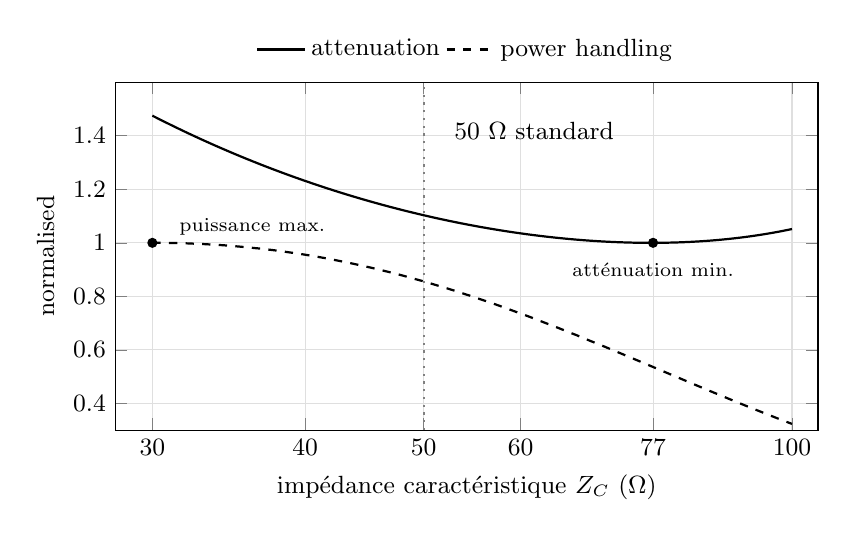
\begin{tikzpicture}
    \begin{axis}[
      width=10.5cm, height=6.0cm,
      xmode=log, log basis x=10,
      xlabel={impédance caractéristique $Z_C$ ($\Omega$)},
      ylabel={normalised},
      xmin=28, xmax=105, ymin=0.3, ymax=1.6,
      xtick={30,40,50,60,77,100},
      xticklabels={30,40,50,60,77,100},
      ytick={0.4,0.6,0.8,1.0,1.2,1.4},
      grid=both, grid style={gray!25},
      legend style={at={(0.5,1.03)},anchor=south,legend columns=2,
                    draw=none,font=\small},
      tick label style={font=\small}, label style={font=\small},
      ]
      \addplot[thick,domain=30:100,samples=90] {((1+exp(x/60))/(x/60))/3.5913};
      \addlegendentry{attenuation}
      \addplot[thick,dashed,domain=30:100,samples=90]
        {((x/60)*exp(-2*x/60))/0.18394};
      \addlegendentry{power handling}
      \draw[gray,dotted,thick] (axis cs:50,0.3) -- (axis cs:50,1.6);
      \node[font=\small,anchor=west] at (axis cs:52,1.42) {$50\ \Omega$ standard};
      \node[circle,fill=black,inner sep=1.3pt] at (axis cs:77,1.0) {};
      \node[font=\scriptsize,anchor=north] at (axis cs:77,0.96)
        {atténuation min.};
      \node[circle,fill=black,inner sep=1.3pt] at (axis cs:30,1.0) {};
      \node[font=\scriptsize,anchor=west] at (axis cs:31,1.06)
        {puissance max.};
    \end{axis}
  \end{tikzpicture}
  \caption*{\small The $50\ \Omega$ compromise for a câble coaxial:
  attenuation is minimum at $Z_C = 77\ \Omega$, power handling is maximum at
  $Z_C = 30\ \Omega$, and $50\ \Omega$ costs about 10~\% of each.}
\end{figure}

\begin{remark}[Physical meaning of $Z_C$ --- read this one twice]
  $Z_C$ n'est \emph{pas} une impédance « matérielle » mais un modèle décrivant
  la distribution de la puissance du signal progressif, à l'abscisse $z$, se
  propageant sur la ligne : cette puissance est distribuée sur la tension
  $V^{+}(z)$ et le courant $I^{+}(z)$ en fonction des dimensions transversales
  et des caractéristiques du matériau diélectrique de la ligne de propagation.
  Equivalently, $Z_C$ est l'impédance qui serait vue en $z = -l$ si la ligne
  était de longueur infinie --- ou fermée par une impédance de charge adaptée
  (c'est-à-dire qu'il n'y a pas de réflexion).
\end{remark}

\subsection{Facteur de réflexion, impédance ramenée, ondes stationnaires}
À noter que l'on va traiter exclusivement le cas de \emph{lignes sans pertes}
($\alpha = 0$, $\gamma = j\beta$) dans ce cours.

\begin{figure}[h!]
  \centering
  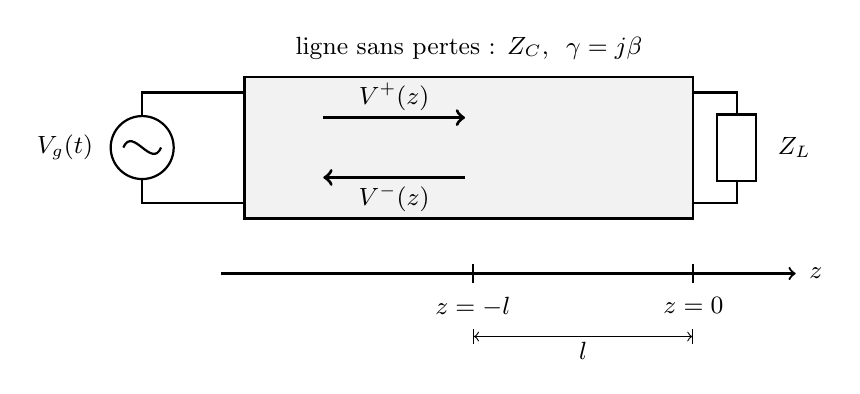
\begin{tikzpicture}[scale=1.0]
    % line body
    \fill[gray!10] (1.3,-0.9) rectangle (7,0.9);
    \draw[thick] (1.3,-0.9) rectangle (7,0.9);
    \node[font=\small,anchor=south] at (4.15,1.0)
      {ligne sans pertes : $Z_C$,\ \ $\gamma = j\beta$};
    \draw[->,very thick] (2.3,0.38) -- node[above,font=\small,inner sep=2pt]
      {$V^{+}(z)$} (4.1,0.38);
    \draw[<-,very thick] (2.3,-0.38) -- node[below,font=\small,inner sep=2pt]
      {$V^{-}(z)$} (4.1,-0.38);
    % generator
    \draw[thick] (0,0) circle (0.4);
    \draw[thick] (-0.24,0) .. controls (-0.12,0.28) and (0.12,-0.28) .. (0.24,0);
    \node[font=\small,anchor=east] at (-0.5,0) {$V_g(t)$};
    \draw[thick] (0,0.4) -- (0,0.7) -- (1.3,0.7);
    \draw[thick] (0,-0.4) -- (0,-0.7) -- (1.3,-0.7);
    % load
    \draw[thick,fill=white] (7.3,-0.42) rectangle (7.8,0.42);
    \node[font=\small,anchor=west] at (7.95,0) {$Z_L$};
    \draw[thick] (7,0.7) -- (7.55,0.7) -- (7.55,0.42);
    \draw[thick] (7,-0.7) -- (7.55,-0.7) -- (7.55,-0.42);
    % axis
    \draw[->,thick] (1.0,-1.6) -- (8.3,-1.6);
    \node[font=\small,anchor=west] at (8.35,-1.6) {$z$};
    \draw[thick] (7,-1.48) -- (7,-1.72);
    \node[font=\small,anchor=north] at (7,-1.78) {$z=0$};
    \draw[thick] (4.2,-1.48) -- (4.2,-1.72);
    \node[font=\small,anchor=north] at (4.2,-1.78) {$z=-l$};
    \draw[|<->|] (4.2,-2.4) -- node[below,font=\small,inner sep=2pt] {$l$} (7,-2.4);
  \end{tikzpicture}
  \caption*{\small The reference configuration. The origin sits at the load, so
  the line lives at $z<0$ and $z=-l$ is a distance $l$ back towards the
  generator.}
\end{figure}

\subsubsection{Facteur de réflexion}
En $z = 0$, la tension et le courant s'écrivent :
\[
  V(z=0) = V_0^{+} + V_0^{-}, \qquad
  I(z=0) = \frac{V_0^{+}}{Z_C} - \frac{V_0^{-}}{Z_C} .
\]
L'existence d'une tension et d'un courant réfléchis le long de la ligne est
dépendante d'une réflexion de l'onde incidente au niveau de l'interface
ligne/impédance de charge en $z=0$.

\begin{definition}[Facteur de réflexion]
  On peut exprimer le \textbf{facteur de réflexion} (\textit{reflection
  coefficient}) à la charge ainsi :
  \[
    \Gamma(z=0) = \frac{V_0^{-}}{V_0^{+}},
  \]
  avec $V_0^{+}$ l'amplitude de la tension incidente et $V_0^{-}$ l'amplitude
  de la tension réfléchie en $z=0$. En $z = -l$, où
  $V(z=-l) = V_0^{+}e^{-j\beta l} + V_0^{-}e^{+j\beta l}$ et
  $I(z=-l) = \left(V_0^{+}e^{-j\beta l} - V_0^{-}e^{+j\beta l}\right)/Z_C$,
  le facteur de réflexion s'écrit alors
  \[
    \Gamma(z=-l) = \frac{V_0^{-}e^{+j\beta l}}{V_0^{+}e^{-j\beta l}}
                 = \frac{V_0^{-}}{V_0^{+}}\,e^{+2j\beta l},
  \]
  et en tout point $z$ de la ligne sans pertes, on peut écrire :
  \[
    \boxed{\; \Gamma(z) = \frac{V_0^{-}}{V_0^{+}}\,e^{+2j\beta z}. \;}
  \]
\end{definition}

On notera le module $|\Gamma(z)| = |V_0^{-}|/|V_0^{+}|$ du facteur de
réflexion, constant along a ligne sans pertes; only the phase changes, and it
changes at twice the rate of a one-way trip --- the déphasage $2\beta z$
accounts for the round trip to the load and back.

\subsubsection{Expression de l'impédance le long d'une ligne ou impédance ramenée}
En $z=0$, l'impédance de charge est liée à la tension et au courant par :
\[
  Z_L = \frac{V(z=0)}{I(z=0)} = Z_C\,\frac{V_0^{+} + V_0^{-}}{V_0^{+} - V_0^{-}}
      = Z_C\,\frac{1+\Gamma(z=0)}{1-\Gamma(z=0)} .
\]

\begin{theorem}[Facteur de réflexion d'une impédance de charge]
  \[
    \boxed{\;
    \Gamma(z=0) = \frac{V_0^{-}}{V_0^{+}} = \frac{Z_L - Z_C}{Z_L + Z_C} .
    \;}
  \]
\end{theorem}

\begin{notation}[Quelques valeurs à retenir]
  Four limiting cases of $\Gamma$ at the load:
  \begin{itemize}
    \item Si $Z_L$ est un \textbf{court-circuit} (\textit{short circuit}, CC),
      $Z_L = 0$ : $\Gamma(z=0) = -1$.
    \item Si $Z_L$ est un \textbf{circuit ouvert} (\textit{open circuit}, CO),
      $Z_L = \infty$ : $\Gamma(z=0) = +1$.
    \item Si $Z_L$ est \textbf{adaptée} (\textit{matched}) à la ligne,
      $Z_L = Z_C$ : $\Gamma(z=0) = 0$ (pas de réflexion).
    \item $-1 \le \Gamma(z=0) \le 1$ (and $0 \le |\Gamma(z=0)| \le 1$ in the
      complex case).
  \end{itemize}
\end{notation}

Pour une ligne sans pertes de longueur $l$, on peut ainsi déterminer
l'\textbf{impédance ramenée} --- the impedance ``brought back'' to $z=-l$ ---
créée par l'impédance de charge $Z_L$ et le tronçon de ligne de propagation de
longueur $l$. The algebra is carried at an arbitrary abscissa $z$ and
specialised to $z=-l$ only at the very end:
\[
  Z(z) = \frac{V(z)}{I(z)}
       = Z_C\,\frac{V_0^{+}e^{-j\beta z} + V_0^{-}e^{+j\beta z}}
                   {V_0^{+}e^{-j\beta z} - V_0^{-}e^{+j\beta z}}
       = Z_C\,\frac{e^{-j\beta z} + \Gamma(z=0)\,e^{+j\beta z}}
                   {e^{-j\beta z} - \Gamma(z=0)\,e^{+j\beta z}} .
\]
En introduisant $\Gamma(z=0) = (Z_L-Z_C)/(Z_L+Z_C)$, l'expression ci-dessus
devient (after clearing the inner denominators) :
\[
  Z(z) = Z_C\,
  \frac{Z_L\left(e^{-j\beta z} + e^{+j\beta z}\right)
        + Z_C\left(e^{-j\beta z} - e^{+j\beta z}\right)}
       {Z_L\left(e^{-j\beta z} - e^{+j\beta z}\right)
        + Z_C\left(e^{-j\beta z} + e^{+j\beta z}\right)} .
\]
$Z(z) = Z_C\left(Z_L - jZ_C\tan(\beta z)\right)/\left(Z_C - jZ_L\tan(\beta z)\right)$
s'obtient en faisant apparaître l'expression des lignes trigonométriques ;
setting $z = -l$ --- which flips the sign of the sines --- gives the result to
remember.

\begin{theorem}[Impédance ramenée]
  Pour une ligne sans pertes d'impédance caractéristique $Z_C$ fermée sur une
  impédance de charge $Z_L$, l'impédance vue à l'abscisse $z = -l$ est
  \[
    \boxed{\;
    Z(z=-l) = Z_C\,
    \frac{Z_L + j\,Z_C\tan(\beta l)}{Z_C + j\,Z_L\tan(\beta l)} .
    \;}
  \]
\end{theorem}

\begin{remark}
  Carried directly in $l$, the collection step reads
  $Z_L(e^{+j\beta l} + e^{-j\beta l}) + Z_C(e^{+j\beta l} - e^{-j\beta l})$
  over $Z_L(e^{+j\beta l} - e^{-j\beta l}) + Z_C(e^{+j\beta l} + e^{-j\beta l})$:
  at $z = -l$ the two exponentials of the route in $z$ swap places, and the
  term in $Z_C$ enters the denominator with a plus sign. Both routes close on
  the box.
\end{remark}

\begin{corollary}[Ligne quart d'onde (\textit{quarter-wave line})]
  Ici $\beta = 2\pi/\lambda$, et une ligne de longueur $l = \lambda/4$ donne
  $\beta l = \pi/2$ et $\tan(\beta l) \to \infty$, d'où l'impédance ramenée
  \[
    \boxed{\; Z(z=-\lambda/4) = \frac{Z_C^{\,2}}{Z_L} . \;}
  \]
  Il s'agit d'un \textbf{transformateur d'impédance} (\textit{impedance
  transformer}). Ce cas particulier sera utilisé au chapitre suivant traitant
  de l'adaptation d'impédance --- it is the basis of the quarter-wave technique
  there.
\end{corollary}

\begin{corollary}
  Si $Z_L = Z_C$, l'impédance présentée en tout point de la ligne est égale à
  l'impédance caractéristique, $Z(z) = Z_C$ (pas d'ondes réfléchies). Le régime
  d'onde est alors appelé \textbf{régime d'onde progressif}
  (\textit{travelling-wave regime}).
\end{corollary}

\subsubsection{Ondes stationnaires}
Selon l'impédance de charge $Z_L$ fermant la ligne de propagation d'impédance
caractéristique $Z_C$, il peut y avoir sur la ligne une onde incidente et une
onde réfléchie. La ligne est parcourue par une onde incidente et une onde
réfléchie, ce qui se traduit par un \textbf{régime d'onde stationnaire}
(\textit{standing-wave regime}), avec la présence de maxima et de minima de
tension le long de la ligne. Quand l'onde incidente \emph{n'est pas} réfléchie
par l'impédance de charge, une simple onde progressive se propage sur la ligne
et la tension ne possède pas d'extremum.

La solution générale complète de la tension sinusoïdale, de pulsation
$\omega = 2\pi F$, se propageant sur la ligne s'écrit :
\[
  V(z,t) = V(z)\,e^{j\omega t}
         = \left(V^{+}(z) + V^{-}(z)\right)e^{j\omega t},
  \qquad
  V^{+}(z) = V^{+}e^{-j\beta z}, \quad V^{-}(z) = V^{-}e^{+j\beta z}.
\]
Le signal résultant provient de la superposition de la tension incidente se
propageant sur l'axe dans le sens des $z$ positifs et de la tension réfléchie
se propageant dans le sens des $z$ négatifs. Over one temporal period
$\Delta t$ the two components run past each other, but the envelope of their
sum is \emph{fixed in space}: the resultant is not a wave that travels, it is a
pattern that breathes in place.

\begin{definition}[Nœuds et ventres]
  Les minima de tension le long de la ligne sont appelés \textbf{nœuds}
  (\textit{node}) ; les maxima de tension sont appelés \textbf{ventres}
  (\textit{antinode}). Les uns et les autres sont \emph{fixes, dans le temps},
  sur l'axe de propagation $Oz$. La distance entre 2 nœuds ou 2 ventres
  successifs est égale à $\lambda/2$.
\end{definition}

\begin{figure}[h!]
  \centering
  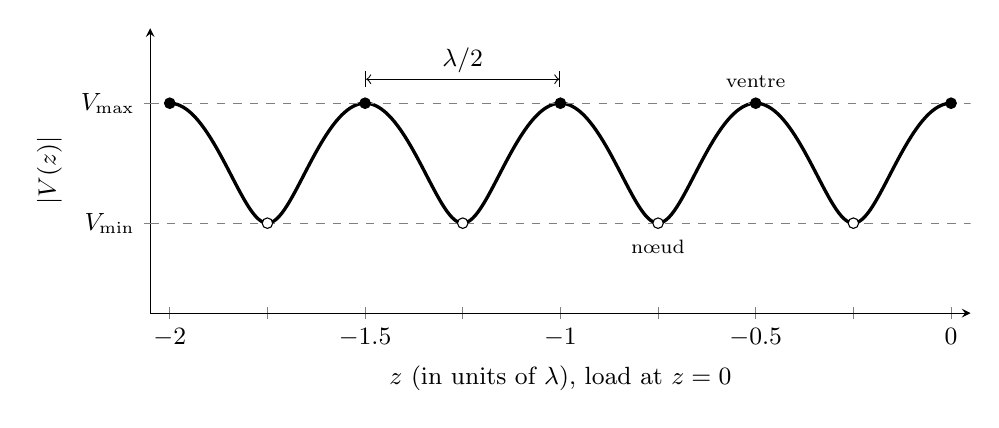
\begin{tikzpicture}
    \begin{axis}[
      width=12cm, height=5.2cm,
      xlabel={$z$ (in units of $\lambda$), load at $z=0$},
      ylabel={$|V(z)|$},
      xmin=-2.05, xmax=0.05, ymin=0, ymax=1.9,
      xtick={-2,-1.75,-1.5,-1.25,-1,-0.75,-0.5,-0.25,0},
      xticklabels={$-2$,,$-1.5$,,$-1$,,$-0.5$,,$0$},
      ytick={0.6,1.4}, yticklabels={$V_{\min}$,$V_{\max}$},
      grid=none, axis lines=left,
      tick label style={font=\small}, label style={font=\small},
      ]
      \addplot[very thick,domain=-2:0,samples=300]
        {sqrt(1.16 + 0.8*cos(720*x))};
      \addplot[only marks,mark=*,mark size=1.9pt]
        coordinates {(0,1.4) (-0.5,1.4) (-1,1.4) (-1.5,1.4) (-2,1.4)};
      \addplot[only marks,mark=*,mark size=1.9pt,fill=white]
        coordinates {(-0.25,0.6) (-0.75,0.6) (-1.25,0.6) (-1.75,0.6)};
      \draw[dashed,gray] (axis cs:-2.05,1.4) -- (axis cs:0.05,1.4);
      \draw[dashed,gray] (axis cs:-2.05,0.6) -- (axis cs:0.05,0.6);
      \draw[|<->|] (axis cs:-1.5,1.56) -- node[above,font=\small,inner sep=2pt]
        {$\lambda/2$} (axis cs:-1,1.56);
      \node[font=\scriptsize,anchor=north] at (axis cs:-0.75,0.55)
        {nœud};
      \node[font=\scriptsize,anchor=south] at (axis cs:-0.5,1.44)
        {ventre};
    \end{axis}
  \end{tikzpicture}
  \caption*{\small Enveloppe de la tension $V^{+}(z)+V^{-}(z)$ le long de la
  ligne de propagation, here for $|\Gamma| = 0{,}4$, so $V_{\max} = 1{,}4$,
  $V_{\min} = 0{,}6$ and $\mathrm{ROS} = 2{,}33$. Nœuds (open) and ventres
  (filled) are fixed in space and spaced by $\lambda/2$.}
\end{figure}

En un ventre, les tensions incidente et réfléchie sont \emph{en phase}, et
l'on a $V_{\max} = |V^{+}| + |V^{-}|$ ; en un nœud, elles sont en opposition de
phase, et l'on a $V_{\min} = |V^{+}| - |V^{-}|$.

\begin{definition}[Rapport d'onde stationnaire (ROS)]
  On caractérise ce phénomène de propagation par le \textbf{rapport d'onde
  stationnaire} (\textit{standing wave ratio}, ROS), VSWR (\textit{Voltage
  Standing Wave Ratio}) en anglais, défini par
  \[
    \mathrm{ROS} = \frac{V_{\max}}{V_{\min}}
                 = \frac{|V^{+}| + |V^{-}|}{|V^{+}| - |V^{-}|} .
  \]
\end{definition}

\begin{theorem}[ROS et $\Gamma$]
  On rencontre un phénomène de propagation par ondes stationnaires lorsque sur
  l'axe de propagation il existe une impédance de charge $Z_L$ différente de
  l'impédance caractéristique $Z_C$ de la ligne. Pour une ligne sans pertes,
  avec le module du facteur de réflexion
  $|\Gamma(z=0)| = |V_0^{-}|/|V_0^{+}| = \left|(Z_L-Z_C)/(Z_L+Z_C)\right|$,
  on peut écrire le ROS ainsi :
  \[
    \boxed{\;
    |\Gamma(z=0)| = \frac{\mathrm{ROS} - 1}{\mathrm{ROS} + 1},
    \qquad
    \mathrm{ROS} = \frac{1 + |\Gamma(z=0)|}{1 - |\Gamma(z=0)|} .
    \;}
  \]
\end{theorem}

À noter que $0 \le |\Gamma(z=0)| \le 1$ et naturellement
$1 \le \mathrm{ROS} < \infty$. Lorsque $\mathrm{ROS} \approx 1$, les impédances
$Z_L$ et $Z_C$ sont identiques : l'impédance de charge est alors adaptée à
l'impédance caractéristique de la ligne, et le maximum de puissance est transmis
et dissipé dans l'impédance de charge. Adaptation : $\mathrm{ROS} = 1$.

\subsubsection{Conséquences sur la puissance délivrée à l'impédance de charge}
Si un générateur RF fournit un signal de puissance de 1~mW à l'entrée d'une
ligne d'impédance caractéristique $Z_C = 50\ \Omega$, la puissance mesurée par
un wattmètre à la sortie, qui simule une impédance de charge, sera de 1~mW car
l'impédance d'entrée du wattmètre est aussi de $50\ \Omega$ : il y a alors
adaptation d'impédance entre l'impédance d'entrée du wattmètre et l'impédance
caractéristique du câble. Si maintenant on remplace la ligne par une ligne
d'impédance caractéristique $Z_C \ne 50\ \Omega$, la puissance mesurée par le
wattmètre sera inférieure à 1~mW, et d'autant plus inférieure que $Z_C$
s'éloigne de la valeur optimale de $50\ \Omega$ : il y a dans ce cas une
\emph{désadaptation d'impédance}.

\begin{example}[1~mW into a $50\ \Omega$ wattmètre through a lossless cable]
  \begin{center}
    \begin{tabular}{cc}
      \toprule
      $Z_C$ du câble & puissance mesurée par le wattmètre \\
      \midrule
      $10\ \Omega$  & $0{,}56$~mW \\
      $20\ \Omega$  & $0{,}82$~mW \\
      $\mathbf{50\ \Omega}$  & $\mathbf{1}$~\textbf{mW} \\
      $100\ \Omega$ & $0{,}89$~mW \\
      \bottomrule
    \end{tabular}
  \end{center}
  The full 1~mW arrives only for $Z_C = 50\ \Omega$.
\end{example}

\begin{remark}
  The rows are what $P = P_{inc}\left(1-|\Gamma_0|^2\right)$ with
  $\Gamma_0 = (50-Z_C)/(50+Z_C)$ predicts, to the digits shown: for the
  $20\ \Omega$ row, for instance, $|\Gamma_0| = 30/70$ gives
  $P = 0{,}82$~mW. The formula is the thing to reproduce.
\end{remark}

Pour une ligne avec pertes (réelle), il faudra ajouter l'atténuation $\alpha$
(on top of this désadaptation loss), mais ça ne sera pas étudié dans ce cours.

\subsection{Puissance transportée dans une ligne sans pertes}
Soit une ligne sans pertes, $\gamma = j\beta$, d'impédance caractéristique
$Z_C$, fermée sur une impédance de charge $Z_L$ quelconque et alimentée par un
générateur RF fournissant un signal $V_g(t)$ sinusoïdal. La tension et le
courant le long de cette ligne s'écrivent :
\[
  V(z) = V^{+}e^{-\gamma z} + V^{-}e^{+\gamma z},
  \qquad
  I(z) = \frac{1}{Z_C}\left(V^{+}e^{-\gamma z} - V^{-}e^{+\gamma z}\right).
\]
La puissance moyenne relevée à l'abscisse $z$ sur la ligne s'écrit :
\[
  P(z) = \Re\!\left[\tfrac{1}{2}\,V(z)\,I^{*}(z)\right].
\]

\begin{proof}
  Avec $\Gamma(z) = \dfrac{V_0^{-}}{V_0^{+}}e^{2j\beta z}$, on peut écrire
  (the voltage and current factorise)
  \[
    V(z) = V^{+}e^{-\gamma z}\left(1 + \Gamma(z)\right),
    \qquad
    I(z) = \frac{1}{Z_C}V^{+}e^{-\gamma z}\left(1 - \Gamma(z)\right),
  \]
  On obtient alors la puissance moyenne :
  \[
    P(z) = \frac{|V^{+}|^{2}}{2Z_C}\,
      \Re\!\left[e^{-(\gamma+\gamma^{*})z}
      \left(1+\Gamma(z)\right)\left(1-\Gamma^{*}(z)\right)\right].
  \]
  La ligne est sans pertes, $\gamma + \gamma^{*} = 0$ --- the exponential
  disappears --- alors :
  \[
    P(z) = \frac{|V^{+}|^{2}}{2Z_C}\,
      \Re\!\left[1 + \Gamma(z) - \Gamma^{*}(z) - \Gamma(z)\Gamma^{*}(z)\right].
  \]
  The middle two terms are purely imaginary and cancel under $\Re$ ; ce qui
  donne :
  \[
    P(z) = \frac{|V^{+}|^{2}}{2Z_C}\left[1 - |\Gamma(z)|^{2}\right]. \qed
  \]
\end{proof}

Le terme $\dfrac{|V^{+}|^{2}}{2Z_C}$ est donc la puissance moyenne transportée
par l'onde incidente. Dans le cas général d'une ligne sans pertes, sur laquelle
se propagent une onde incidente et une onde réfléchie, la puissance consommée
par l'impédance de charge dépend du seul module du facteur de réflexion
$|\Gamma(z=0)|$ :
\[
  P(z=0) = P_{inc}(z=0) - P_{ref}(z=0),
  \qquad
  P_{inc}(z=0) = \frac{|V_0^{+}|^{2}}{2Z_C},
  \qquad
  P_{ref}(z=0) = |\Gamma(z)|^{2}\,\frac{|V_0^{+}|^{2}}{2Z_C}.
\]
Si la ligne est sans pertes, la puissance incidente correspond à la puissance
délivrée par le générateur RF, et $|\Gamma(z)| = |\Gamma(z=0)| \equiv
|\Gamma_0|$ ne dépend pas de $z$.

\begin{theorem}[Bilan de puissance]
  Pour une ligne sans pertes d'impédance caractéristique $Z_C$ fermée sur une
  impédance de charge $Z_L$, la puissance moyenne réfléchie par la charge et la
  puissance moyenne absorbée par la charge s'écrivent
  \[
    \boxed{\;
    P_{ref} = |\Gamma_0|^{2}\,P_{inc},
    \qquad
    P = P_{inc}\left[1 - |\Gamma_0|^{2}\right],
    \qquad
    \Gamma_0 = \frac{Z_L - Z_C}{Z_L + Z_C},
    \;}
  \]
  avec $P_{inc}$ la puissance moyenne fournie par le générateur.
\end{theorem}

\begin{conclusion}
  A désadaptation costs power twice over: the fraction $|\Gamma_0|^2$ of the
  incident power never reaches the load at all, and the onde réfléchie that
  carries it back up the line disturbs the line and the functioning of the
  system feeding it. This is why the next chapter is about adaptation
  d'impédance.
\end{conclusion}

\subsection{Quelques références de valeur de puissance}
La puissance est exprimée en watts (W). Dans le domaine des systèmes RF et
hyperfréquences, on exprimera plus naturellement la puissance dans l'échelle
logarithmique, soit en dBm, soit en dBW.

\begin{definition}[dBm et dBW]
  \[
    P_{\mathrm{dBm}} = 10\log_{10}\left(P_{\mathrm{mW}}\right),
    \qquad
    P_{\mathrm{dBW}} = 10\log_{10}\left(P_{\mathrm{W}}\right),
  \]
  où $P_{\mathrm{mW}}$ est la puissance exprimée en milliwatts et
  $P_{\mathrm{W}}$ la puissance exprimée en watts. On utilise le dBm pour les
  communications sans fil terrestres à courtes et moyennes distances ($<2$ ou
  3~km), entraînant des puissances maximales de l'ordre du watt ; on utilise le
  dBW pour les communications par satellites ou les radars, pour des distances
  $>10$~km où de fortes puissances sont utilisées, de l'ordre de plusieurs
  dizaines de watts à centaines de kilowatts.
\end{definition}

\begin{center}
  \begin{tabular}{ccc}
    \toprule
    Puissance en W & Puissance en dBm & Puissance en dBW \\
    \midrule
    $0{,}1$~mW & $-10$~dBm & $-40$~dBW \\
    $1$~mW     & $0$~dBm   & $-30$~dBW \\
    $10$~mW    & $10$~dBm  & $-20$~dBW \\
    $20$~mW    & $13$~dBm  & $-17$~dBW \\
    $100$~mW   & $20$~dBm  & $-10$~dBW \\
    $1$~W      & $30$~dBm  & $0$~dBW \\
    \bottomrule
  \end{tabular}
\end{center}

On peut ainsi extrapoler facilement à plusieurs centaines de watts, et on
remarque aussi que
\[
  \boxed{\; P_{\mathrm{dBm}} = P_{\mathrm{dBW}} + 30\ \mathrm{dB}. \;}
\]

\begin{example}[Orders of magnitude for WiFi]
  À l'émission, la puissance maximale ne peut dépasser (norme standardisée)
  100~mW, soit 20~dBm. En réception, les valeurs de puissance sont comprises
  entre $-30$ et $-90$~dBm. À $-30$~dBm, la puissance de réception est
  excellente ; entre $-50$ et $-60$~dBm, la qualité du réseau sans fil est
  qualifiée de correcte et la puissance est suffisante pour une activité
  « normale » sur internet ; à $-90$~dBm, la connexion est réellement mauvaise,
  et il est probable que l'on ne pourra pas se connecter.
\end{example}

\subsection{Étude de la ligne coaxiale}
The same results can be established from the fields rather than from a circuit
model --- une démonstration du passage de la notion champ électrique/champ
magnétique à la notion tension/courant se propageant le long d'une ligne
coaxiale --- and the intermediate results are worth keeping. Les conducteurs
sont constitués de métal parfait supposé sans pertes ; le diélectrique
intérieur est supposé linéaire et isotrope, avec pour paramètres constitutifs
$\varepsilon = \varepsilon' - j\varepsilon''$ et $\mu$.

\begin{example}[From Maxwell in cylindrical coordinates to the équations des télégraphistes]
  \textbf{Mode TEM et symétrie azimutale.} Pour un mode TEM, les 2 champs sont
  transverses, ce qui implique $E_z = H_z = 0$ ; la symétrie azimutale rend les
  champs invariants selon la coordonnée $\varphi$ : $\partial/\partial\varphi = 0$.
  L'équation de Maxwell--Ampère, en l'absence de courant de conduction,
  s'écrit $\curl \v{H} = j\omega\varepsilon\v{E}$, et l'équation de
  Maxwell--Faraday $\curl \v{E} = -j\omega\mu\v{H}$ ; le rotationnel d'un
  vecteur quelconque, en coordonnées cylindriques, s'écrit
  \[
    \curl \v{V} =
      \left[\frac{1}{\rho}\frac{\del V_z}{\del \varphi}
            - \frac{\del V_\varphi}{\del z}\right]\unitv{u}_\rho
    + \left[\frac{\del V_\rho}{\del z}
            - \frac{\del V_z}{\del \rho}\right]\unitv{u}_\varphi
    + \frac{1}{\rho}\left[\frac{\del (\rho V_\varphi)}{\del \rho}
            - \frac{\del V_\rho}{\del \varphi}\right]\unitv{u}_z
  \]
  et, en projetant sur $\unitv{u}_z$, on obtient
  $\frac{1}{\rho}\frac{\del(\rho H_\varphi)}{\del\rho} = j\omega\varepsilon E_z = 0$
  et
  $\frac{1}{\rho}\frac{\del(\rho E_\varphi)}{\del\rho} = -j\omega\mu H_z = 0$,
  d'où
  \[
    \rho H_\varphi = g(z), \qquad \rho E_\varphi = f(z),
    \qquad \text{and, on } \unitv{u}_\rho, \quad \rho E_\rho = h(z).
  \]

  \textbf{Conditions de continuité des champs.} Le champ tangentiel est nul sur les parois
  du métal supposé parfait en $\rho = a$ et $\rho = b$ pour tout $z$, d'où
  $E_\varphi = f(z)/a = f(z)/b = 0$, donc $E_\varphi = 0$ et, d'après
  $\del E_\varphi/\del z = j\omega\mu H_\rho$, $H_\rho = 0$. What survives is a
  radial $\v{E}$ and an azimuthal $\v{H}$; finalement les équations de Maxwell
  s'écrivent :
  \[
    \frac{\del h(z)}{\del z} = -j\omega\mu\, g(z),
    \qquad
    \frac{\del g(z)}{\del z} = -j\omega\varepsilon\, h(z).
  \]

  \textbf{Équivalence de la description en champs avec la description en
  courant tension $V$ et $I$.} Dans le plan transverse, le potentiel
  vecteur n'a pas de composante transverse, donc on aura alors
  $\v{E} = -\grad V$ simplement, et
  \[
    V(z) = \int_a^b E_\rho\, d\rho = h(z)\ln\!\left(\frac{b}{a}\right),
    \qquad
    I(z) = \oint \v{H}\cdot d\v{l} = \int_0^{2\pi} H_\varphi\,\rho\, d\varphi
         = 2\pi\, g(z),
  \]
  la seconde en calculant la circulation sur un cercle de rayon $a$ (théorème
  d'Ampère). En injectant ces expressions dans les équations couplées, on
  obtient les équations des télégraphistes
  \[
    dV(z) = -j\omega L\, I(z)\, dz,
    \qquad
    dI(z) = -(G + j\omega C)\, V(z)\, dz,
  \]
  with exactly the éléments distribués the circuit model postulates:
  \[
    L = \frac{\mu\ln(b/a)}{2\pi},
    \qquad
    C = \frac{2\pi\varepsilon'}{\ln(b/a)},
    \qquad
    G = \frac{2\pi\omega\varepsilon''}{\ln(b/a)} .
  \]
\end{example}

\begin{remark}[What the derivation adds]
  Three things beyond the circuit model. First, $G$, qui représente les pertes
  diélectriques, is tied to the imaginary part $\varepsilon''$ of the
  permittivité, so ``pertes diélectriques'' and
  $\tan\delta = \varepsilon''/\varepsilon'$ are the same statement. Second, in
  the lossless case ($G=0$) the constante de propagation
  $\gamma = 0 + j\omega\sqrt{LC}$ obtained on the line est \emph{la même} que
  celle qui serait obtenue dans le diélectrique illimité --- the line does not
  change the physics of the medium, it only channels it. Third, the physical
  model is not unique: many models en éléments localisés reproduce the same
  equations, and dans le cas d'un métal à pertes, une résistance série
  viendrait s'ajouter avec l'inductance $L$.
\end{remark}

\begin{prop}[Vitesse de phase et longueur d'onde dans la ligne]
  \[
    v_\varphi = \frac{\omega}{\beta} = \frac{1}{\sqrt{\varepsilon\mu}},
    \qquad
    \lambda = v_\varphi T = \frac{2\pi}{\beta},
  \]
  valeurs qui sont aussi celles qui seraient obtenues dans le diélectrique
  illimité. L'impédance caractéristique s'obtient en dérivant les solutions
  générales et en identifiant :
  $Z_C = V_0^{+}/I_0^{+} = -V_0^{-}/I_0^{-} = \sqrt{L/C}$.
\end{prop}

\begin{remark}
  Quand il n'y a pas d'ondes réfléchies, $V_0^{-} = I_0^{-} = 0$, et dans ce
  cas l'impédance vue le long de la ligne est constante quel que soit $z$, et
  elle est égale à l'impédance caractéristique $Z_C$. This is the operational
  content of the ``physical meaning of $Z_C$'' remark: $Z_C$ is what an
  infinitely long line --- or one closed on a charge adaptée --- presents.
\end{remark}

\begin{remark}[Why $\Gamma$ and not $V$ is what gets measured]
  Il est extrêmement difficile et coûteux (voire impossible pour des fréquences
  supérieures à 100~GHz) de mesurer la tension pour des fréquences élevées. Le
  facteur de réflexion permet, dans la pratique, de caractériser des
  dispositifs sous test : sa mesure est basée sur la mesure de la puissance
  réfléchie à l'interface d'un dispositif (ou charge) et de la ligne de
  propagation amenant le signal. Cette méthode est réalisable, à relativement
  bas coût, jusqu'à des fréquences extrêmement élevées (quelques THz) --- which
  is why $\Gamma$, and the paramètres S built from it in the next chapter, is
  the currency of RF characterisation.
\end{remark}
